\documentclass{article}

\usepackage{amsmath, amsthm, amssymb, amsfonts}
\usepackage{thmtools}
\usepackage{graphicx}
\usepackage{setspace}
\usepackage{geometry}
\usepackage{float}
\usepackage{hyperref}
\usepackage[utf8]{inputenc}
\usepackage[english]{babel}
\usepackage{framed}
\usepackage[dvipsnames]{xcolor}
\usepackage{tcolorbox}
\usepackage{physics}

\colorlet{LightGray}{White!90!Periwinkle}
\colorlet{LightOrange}{Orange!15}
\colorlet{LightGreen}{Green!15}

\newcommand{\HRule}[1]{\rule{\linewidth}{#1}}

\declaretheoremstyle[name=Theorem,]{thmsty}
\declaretheorem[style=thmsty,numberwithin=section]{theorem}
\tcolorboxenvironment{theorem}{colback=LightGray}

\declaretheoremstyle[name=Proposition,]{prosty}
\declaretheorem[style=prosty,numberlike=theorem]{proposition}
\tcolorboxenvironment{proposition}{colback=LightOrange}

\declaretheoremstyle[name=Principle,]{prcpsty}
\declaretheorem[style=prcpsty,numberlike=theorem]{principle}
\tcolorboxenvironment{principle}{colback=LightGreen}

\setstretch{1.2}
\geometry{
    textheight=9in,
    textwidth=5.5in,
    top=1in,
    headheight=12pt,
    headsep=25pt,
    footskip=30pt
}

% ------------------------------------------------------------------------------

\begin{document}

% ------------------------------------------------------------------------------
% Cover Page and ToC
% ------------------------------------------------------------------------------


% ------------------------------------------------------------------------------



\section*{Points in 2-space, 3-space, and Beyond}

In the same way that we can specify a point in the plane with 
two numbers, we can specify a point in space with three numbers
$(x,y,z)$. In general, in $n$-space ($\mathbb{R}^n$), we can specify
a point with a list of $n$ numbers $(x_1,\ldots,x_n)$.

Given two points in $\mathbb{R}^3$, we can define addition on them 
by adding corresponding coordinates:
\[(a_1,a_2,a_3)+(b_1,b_2,b_3):=(a_1+b_1, a_2+b_2, a_3+b_3).\]
In general,
\[(a_1,\ldots,a_n)+(b_1,\ldots,b_n):=(a_1+b_1,\ldots,a_n+b_n).\]

\textbf{Example.}
Let $A=(2,3)$, $B=(-1,1)$. Then $A+B=(1,4)$.
The figure looks like a parallelogram.

\textbf{Example.}
Let $A=(3,1)$, $B=(1,2)$. Then $A+B=(4,3)$.
We obtain a parallelogram again. This is always the case.
Starting from the origin $O=(0,0)$, we obtain $B$ by moving $1$
unit right and then $2$ units up. We get $A+B$ by first moving 
$3$ to the right, then $1$ up, and then repeating the same movement 
we did from the origin to $B$. In other words, the segment connecting
$O$ to $B$ and the one connecting $A$ to $A+B$ are equal length and parallel.
Similarly, the segments from $O$ to $A$ and $B$ to $B+A = A+B$ will also be equal length and parallel.

We have some not-so-surprising properties of point addition
\begin{itemize}
    \item $(A+B)+C=A+(B+C)$
    \item $A + B = B + A$
    \item $O + A = A + O = A$
    \item $A + (-A) = O$
\end{itemize}
where $O=(0,\ldots,0)$ and $-A = (-a_1, \ldots, -a_n)$.
We note that $A \mapsto -A$ corresponds to reflection about the origin.

We can also multiply (or \emph{scale}) a point $A=(a_1,\ldots,a_n)$ by a number $c$, yielding a point
\[cA = (ca_1, \ldots, ca_n).\]
For example, if $A=(2,-1,5)$ and $c=7$, then $cA=(14,-7,35)$.
We again have some easy properties:
\begin{itemize}
    \item $c(A+B)=cA + cB$
    \item $(c_1 + c_2)A = c_1 A + c_2 A$
    \item $(c_1 c_2)A = c_1(c_2 A)$.
\end{itemize}
We should comment on the geometric meaning of scaling by a number $c$. 
Let $A=(1,2)$ and $c=3$. Then $cA=(3,6)$. We see that the effect of multiplying by $3$ is to
stretch the point $A$ away from the origin by a factor of $3$. If we set $c=1/2$, this 
shrinks $A$ in towards the origin. If we draw a segment from the origin to $A$, in the former case,
scaling by $c=3$ multiplies the length by $3$, and scaling by $c=1/2$ cuts the length in half.

\section*{Vectors}
The discussion above leads us naturally to vectors. Given two points $A$ and $B$,
we can define a \textbf{located vector} as an ordered pair of points $(A,B)$, which is more
often written $\overrightarrow{AB}$. We think of this as an arrow connecting $A$ and $B$,
pointing towards $B$. Two located vectors $\overrightarrow{AB}$ and $\overrightarrow{CD}$
are said to be \textbf{equivalent} if $B-A=D-C$. We always have that
$\overrightarrow{AB}$ is equivalent to $\overrightarrow{O(B-A)}$. This is actually the unique
vector starting at the origin that is equivalent to $\overrightarrow{AB}$.

$\overrightarrow{AB}$ and $\overrightarrow{PQ}$ are said to be \textbf{parallel} if 
for some $c\neq 0$, we have $A-B = c(Q-P)$. If $c>0$ we say the vectors have the \emph{same direction},
and if $c<0$, we say they have the \emph{opposite direction}. 

$\overrightarrow{AB}$ and $\overrightarrow{PQ}$ are said to be \textbf{perpendicular} if 
$B - A$ and $Q - P$ are perpendicular in the usual geometric sense.

A located vector starting from the origin is completely determined by its
endpoint. So an $n$-tuple will be called either a point or a \textbf{vector}
depending on the context and interpretation. 

\section*{The Dot Product}

If $\vec{x} = (x_1,x_2, \ldots, x_n)$ and $\vec{y} = (y_1, y_2, \ldots, y_n)$,
their \textbf{dot product} is 
\[\vec{x} \cdot \vec{y} = x_1 y_1 + x_2 y_2 + \cdots + x_n y_n.\]
Note 

Some useful properties are

\begin{enumerate}
    \item $A \cdot B = B \cdot A$
    \item $A \cdot (B + C) = A \cdot B + A \cdot C = (B+C) \cdot A$
    \item If $x$ is a number, $(xA) \cdot B = x(A \cdot B)$, $A \cdot (xB) = x(A \cdot B)$
    \item If $A=O$, then $A \cdot A = 0$. Otherwise, $A \cdot A > 0$.
\end{enumerate}

Two vectors $A$ and $B$ are said to be \textbf{perpendicular} or \textbf{orthogonal} if
$A \cdot B = 0$. For the plane and $\mathbb{R}^3$, we will see that this
definition agrees with our previous and more geometric definition of perpendicular.

The \textbf{norm} or \textbf{magnitude} (or \textbf{length}) $\norm{A}$ of a vector $A=(a_1, \ldots, a_n)$ is 
\[\norm{A} = \sqrt{A \cdot A} = \sqrt{a_1^2 + \cdots + a_n^2}.\]

Note that $\norm{-A} = \norm{A}$. More generally, for any number $c$, 
we have $\norm{cA} = |c|\norm{A}$. For two points $A,B$, the \textbf{distance}
between them is 
\[\norm{A-B}= \sqrt{(A-B)\cdot(A-B)}.\]

A vector $E$ is a \textbf{unit vector} if $\norm{E}=1$. Dividing a nonzero vector by its norm always yields
a unit vector, since 
\[\norm{\frac{A}{\norm{A}}} = \frac{1}{\norm{A}} \norm{A} = 1.\]

Two nonzero vectors $A$ and $B$ have the \textbf{same direction} if there is some $c>0$ such that
$cA = B$. So, for instance, $A/\norm{A}$ is a unit vector in the same direction as $A$.

\section*{Perpendicularity, Angle Between Vectors}

We have two notions of ``perpendicular'' floating around. One says $A$ and $B$ are perpendicular if $A \cdot B = 0$.
The other is the more familiar notion of $A$ and $B$ forming a right angle. Suppose that $A$ and $B$ lie in the plane.
We can convince ourselves that $A$ and $B$ form a right angle precisely when
\[\norm{A-B} = \norm{A+B}.\]

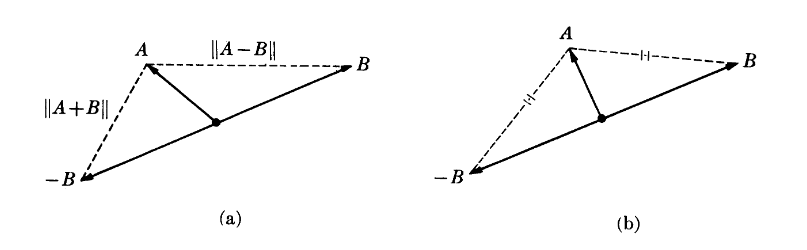
\includegraphics[scale = 0.5]{perpendicular.PNG}

If we accept this, then the equivalence of our two definitions of perpendicularity will follow from 
\[\norm{A+B}=\norm{A-B} \iff A \cdot B = 0.\]

To prove this, observe that
\begin{align*}
    \norm{A+B}=\norm{A-B}&\iff \norm{A + B}^2 = \norm{A - B}^2\\
    &\iff A\cdot A + 2 A \cdot B + B \cdot B = A \cdot A - 2 A \cdot B + B \cdot B\\
    &\iff 4 A \cdot B = 0\\
    &\iff A \cdot B = 0.
\end{align*}

Suppose again that we have two nonzero vectors $A$ and $B$ in the plane, located at the origin.
If we move along the line through $\overrightarrow{OB}$, there will be some point $P$ on this line such
that $\overrightarrow{PA}$ is perpendicular to $\overrightarrow{OB}$. Then $P = c B$ for some number $c$.
Then we have $(A - P)\cdot B = (A - cB)\cdot B = 0$, which is to say
\[A \cdot B - c B \cdot B = 0,\]
so that
\[c = \frac{A \cdot B}{B \cdot B}.\]

Conversely, we see that
\[\left( A - \frac{A \cdot  B}{B \cdot B} B \right) \cdot B = A\cdot B - A \cdot B = 0.\]
Thus, this is the unique number $c$ that makes $A - cB$ perpendicular to $B$. This number $c$ is called
the \textbf{component} of $A$ along $B$. If we do a little plane geometry, we see that
\[\cos \theta = \frac{c \norm{B}}{\norm{A}},\]
which can be rewritten as 
\[\norm{A} \norm{B} \cos \theta = A \cdot B.\]
% ------------------------------------------------------------------------------
\end{document}